\begin{appendices}
	\clearpage
	\pagenumbering{roman}	
	\chapter{Periodensystem}

	% http://commons.wikimedia.org/wiki/File:Periodic_table_simple_de_bw.svg
	\begin{figure}\label{fig:persys}
	\centering
	\includegraphics[width=\textwidth]{../fig/periodensystem_1.pdf}
	\end{figure}	

	\begin{figure}
	\centering
	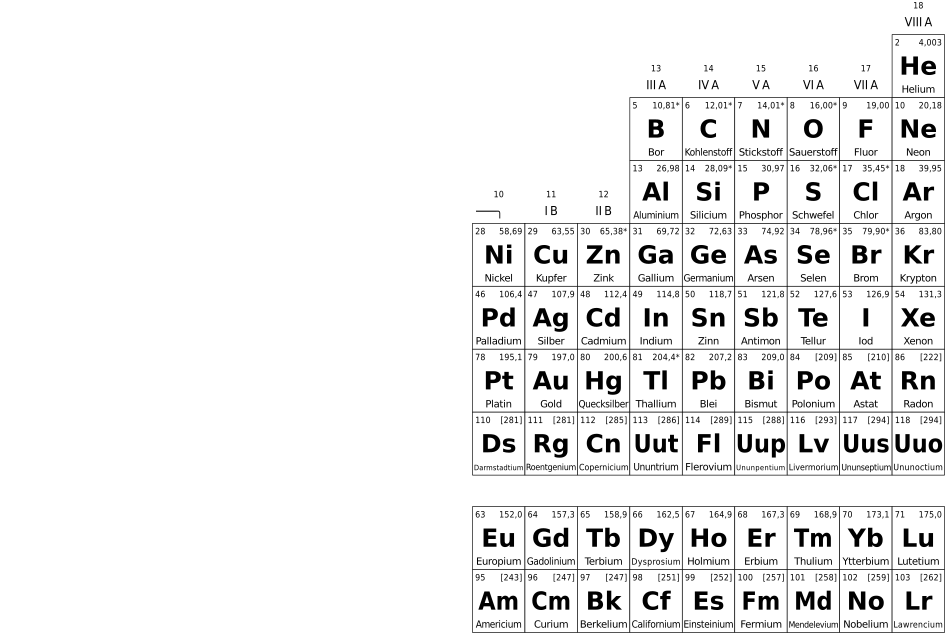
\includegraphics[width=\textwidth]{../fig/periodensystem_2.pdf}
	\end{figure}

	\chapter{STM32F21xx}\label{sec:stm32f21xx}
	Der Mikrocontroller STM32F21xx ist ein repräsentatives Modell von
	Mikrocontrollern, welche heutzutage für Embedded Systems benutzt 
	werden im Bereich der Steuereungs- und Retgelungstechnik. Die 
	typischen Merkmale solcher Mikrocontroller sind
	\begin{itemize}
		\item 32-Bit Busbreite
		\item RISC-Architektur (aktuell z.B. ARM-Cores mit Thumb2)
		\item diverse interne Peripheriecontroller (UART, SPI, I$^2$C, Ethernet)
		\item DMA (Direct Memory Access)
		\item ADC (Analog to Digital Converter)
		\item Pipelining (Sprungvorhersagen)
		\item Single Cycle Multiplication
	\end{itemize}

	\newpage
	\section{ADC Genauigkeit}\label{sec:stm32f21xx-adc}
	\begin{figure}[h!]
		\centering
		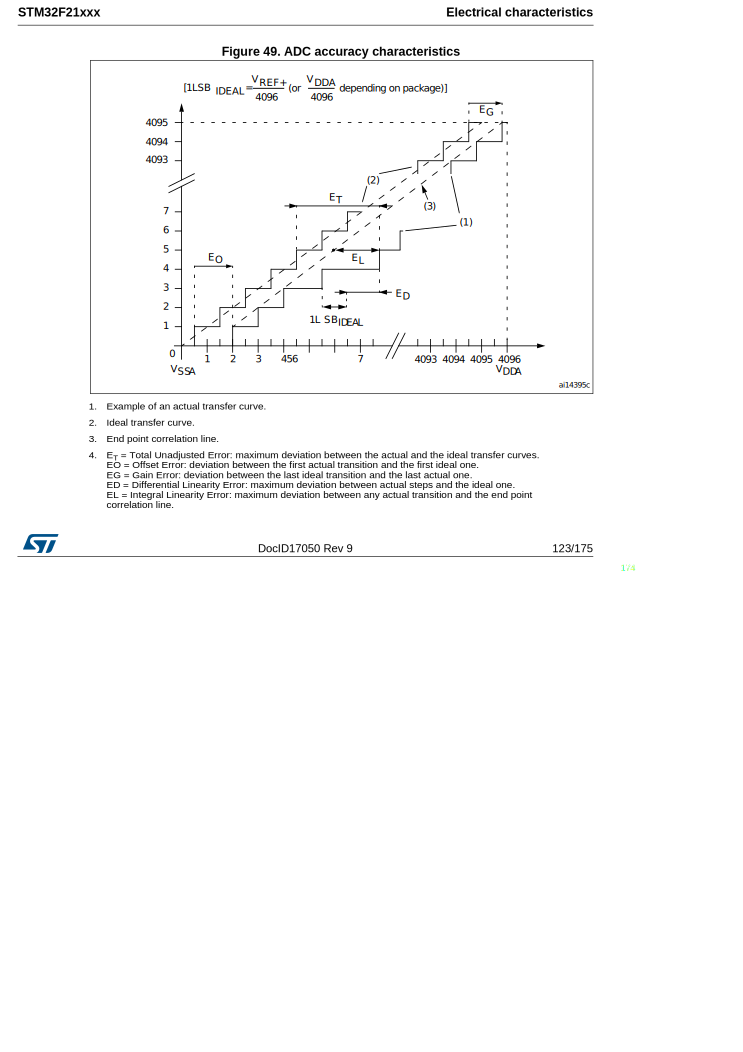
\includegraphics[width=1\textwidth]{../fig/stm32f21xx-adc.pdf}
	\end{figure}

	\newpage
	\section{Jitter PLL}
	\begin{figure}[h!]
		\centering
		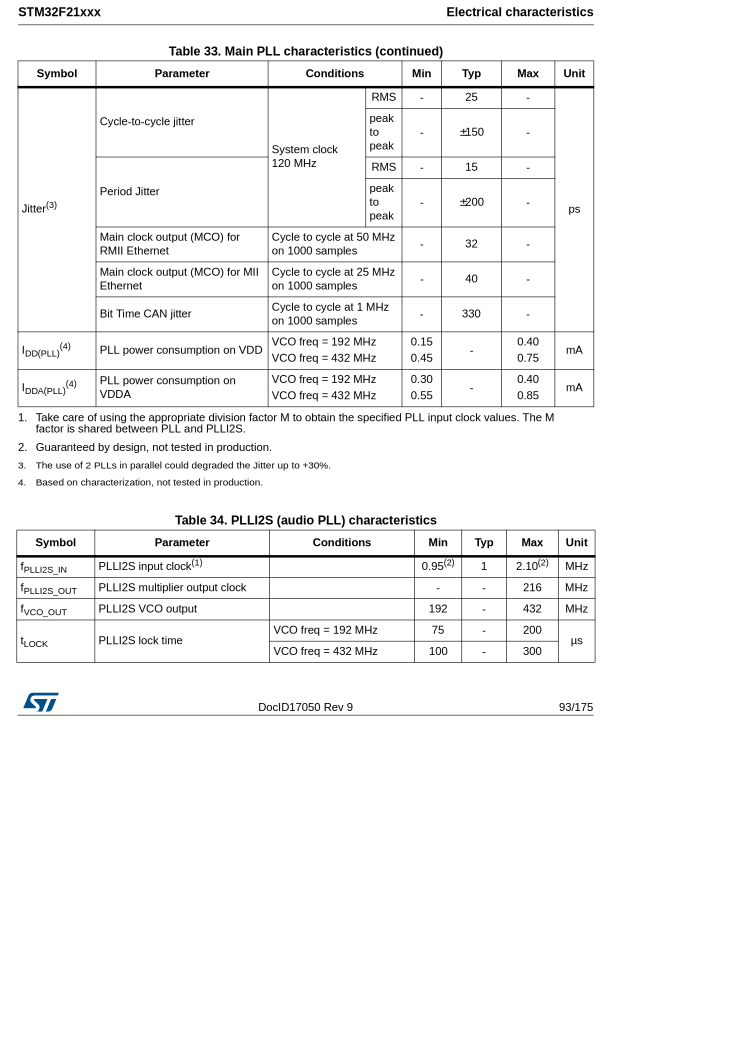
\includegraphics[width=1\textwidth]{../fig/stm32f21xx-jitter-pll.pdf}
	\end{figure}
	
	\newpage
	\section{Jitter Audio-PLL}
	\begin{figure}[h!]
		\centering
		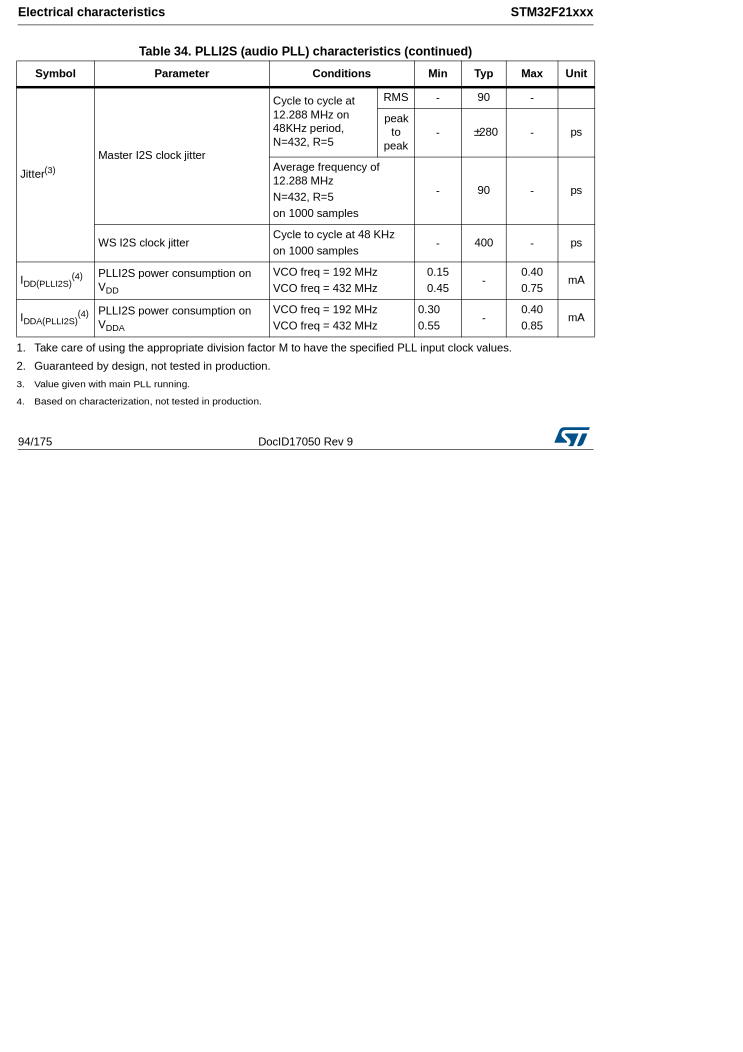
\includegraphics[width=1\textwidth]{../fig/stm32f21xx-jitter-audio-pll.pdf}
	\end{figure}
\end{appendices}
